\begin{figure}[!tb]
  \centering
  \begin{subfigure}{0.55\linewidth}
    \centering
    \caption{}
    \label{subfig:visual_abstract_1}
  \vspace{-1.3\baselineskip}
  \begin{minipage}[t]{0.33\linewidth}
    \centering
    % load "spectrumdefault{left, center, right}" styles
    % defines the pgfplots styles "spectrumdefault", "spectrumdefaultleft",
% "spectrumdefaultcenter", "spectrumdefaultright"
% pgfplots style "spectrumdefault"
\pgfkeys{/pgfplots/spectrumdefault/.style={
    width=1.38\linewidth,
    height=1.38*1.8\linewidth,
    every axis plot/.append style={line width = 1.5pt},
    tick pos = left,
    xmajorticks = true,
    ymajorticks = true,
    ylabel near ticks,
    xlabel near ticks,
    xtick align = inside,
    ytick align = inside,
    legend cell align = left,
    legend columns = 1,
    legend pos = north west,
    legend style = {
      fill opacity = 0.7,
      text opacity = 1,
      font = \footnotesize,
    },
    xticklabel style = {font = \footnotesize, inner xsep = 0ex},
    xlabel style = {font = \footnotesize},
    axis line style = {black},
    yticklabel style = {font = \footnotesize, inner ysep = 0ex},
    ylabel style = {font = \footnotesize, inner ysep = 0ex},
    title style = {font = \footnotesize, inner ysep = 0ex, yshift = -0.75ex},
    grid = major,
    grid style = {dashed}
  }
}
% pgfplots style for left "spectrumdefaultleft"
\pgfkeys{/pgfplots/spectrumdefaultleft/.style={
    spectrumdefault,
    title=\empty,
    ymax=3e-4,
    xlabel=\phantom{eigenvalues},
  }}
% pgfplots style for center "spectrumdefaultcenter"
\pgfkeys{/pgfplots/spectrumdefaultcenter/.style={
    spectrumdefault,
    ylabel=\empty,
    yticklabels=\empty,
    title=\empty,
    ymax=3e-4,
  }}
% pgfplots style for right "spectrumdefaultright"
\pgfkeys{/pgfplots/spectrumdefaultright/.style={
    spectrumdefault,
    ylabel=\empty,
    yticklabels=\empty,
    title=\empty,
    ymax=3e-4,
    xlabel=\phantom{eigenvalues},
  }}

%%% Local Variables:
%%% mode: latex
%%% TeX-master: "../../thesis"
%%% End:

    % customize "zmystyle" as you wish
    \pgfkeys{/pgfplots/zmystyle/.style={spectrumdefaultleft,
        title={mb, exact}}}
    % This file was created by tikzplotlib v0.9.7.
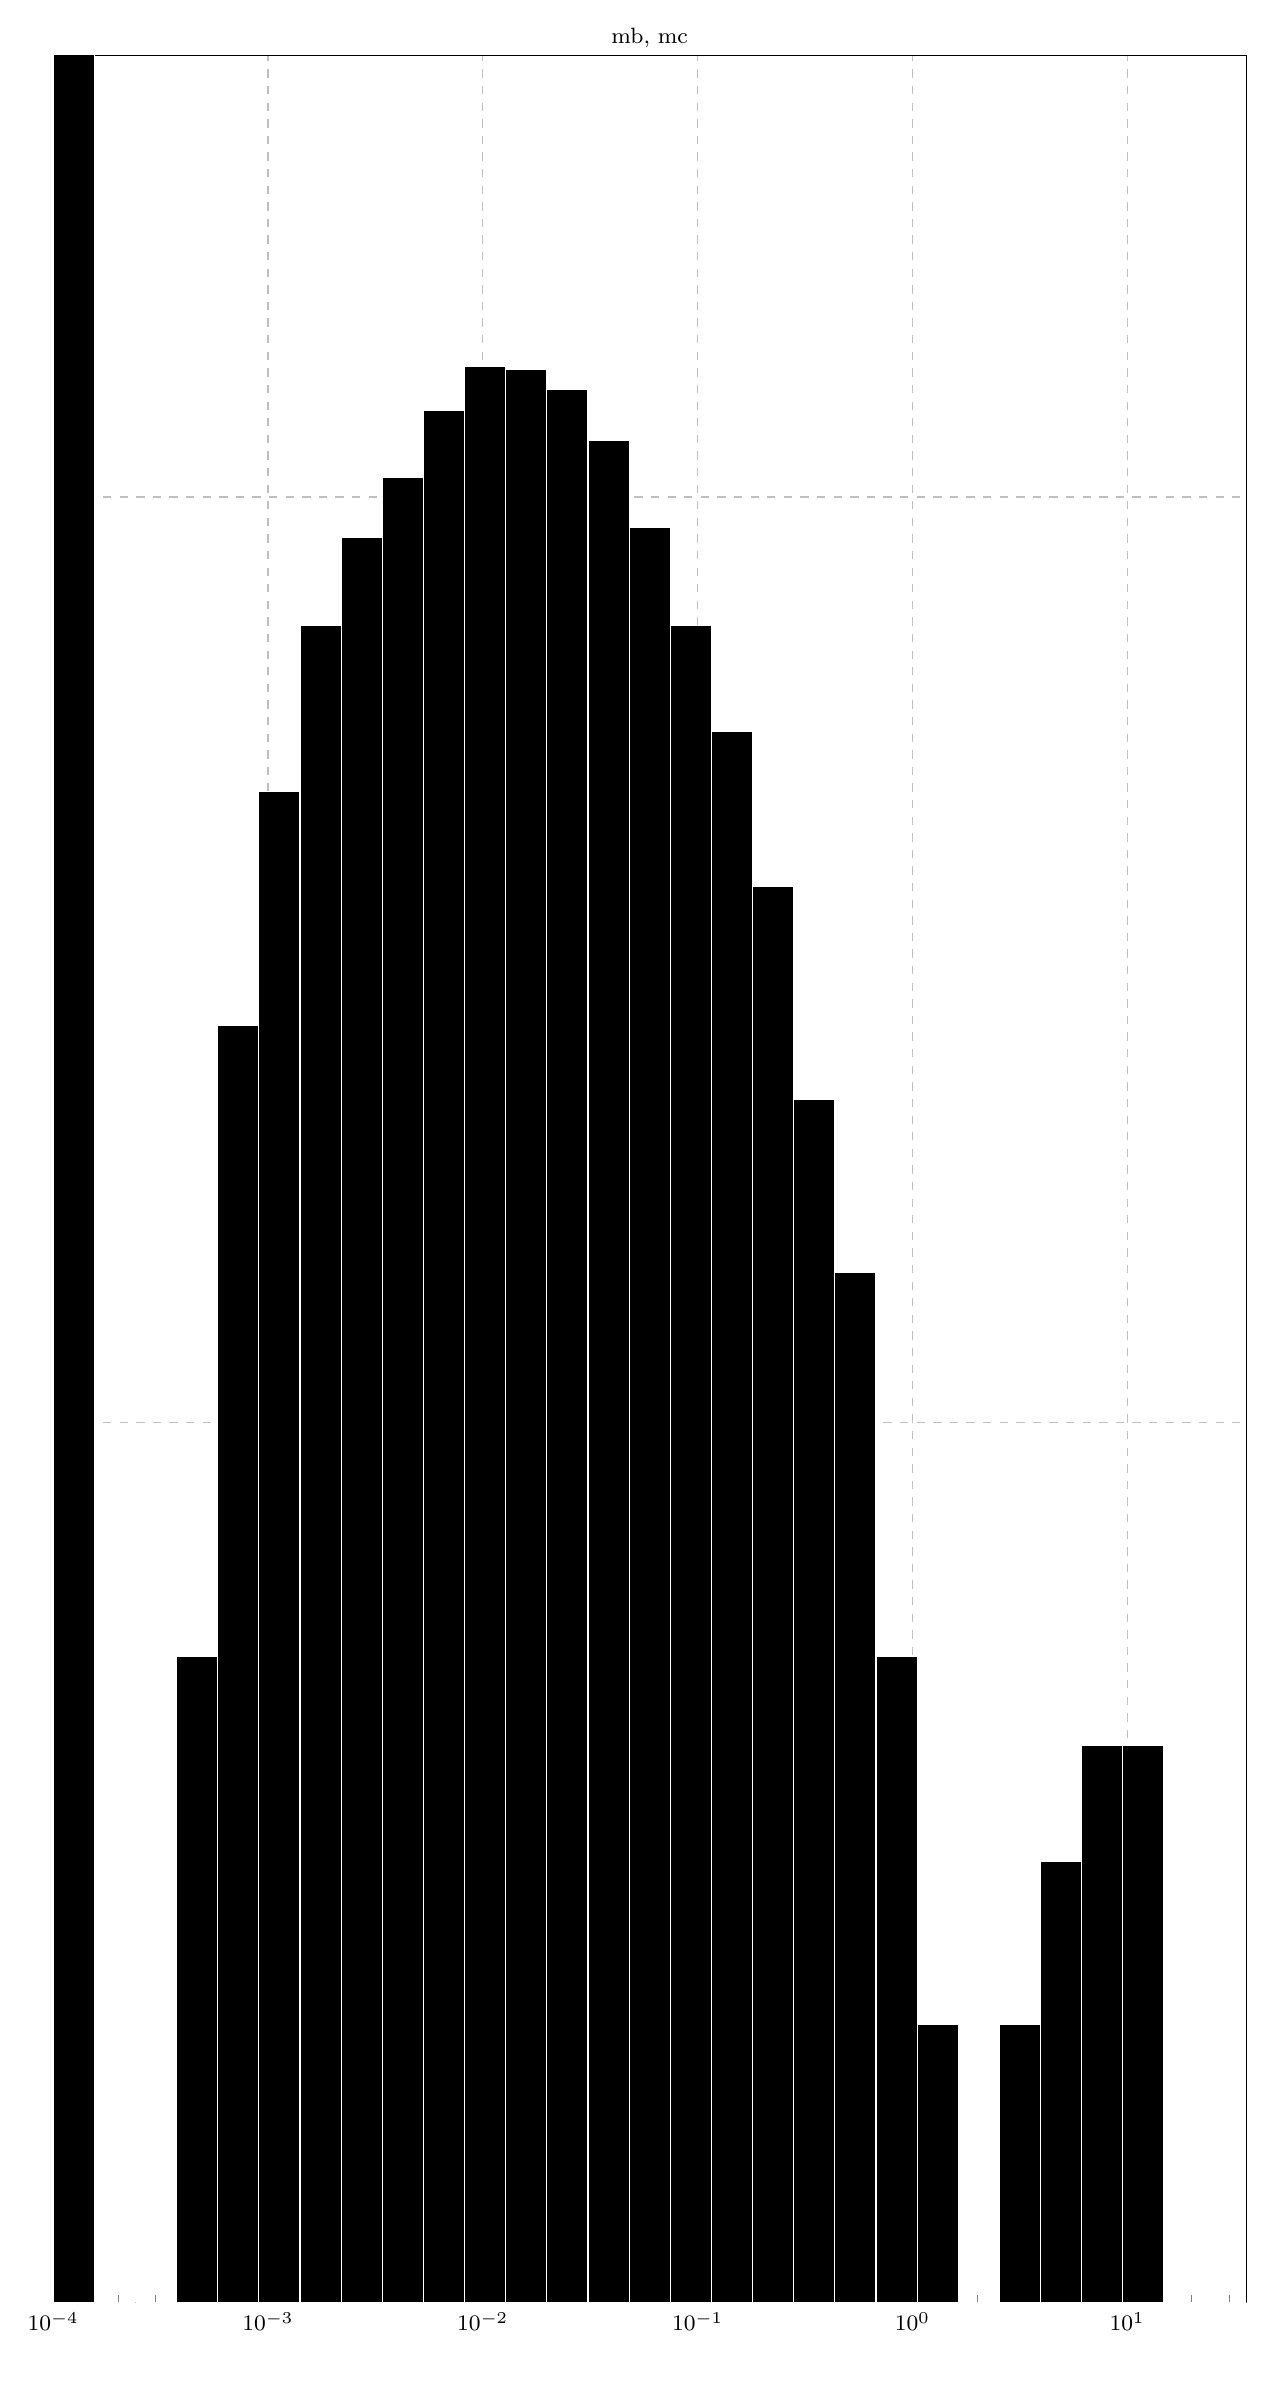
\begin{tikzpicture}

\begin{axis}[
axis line style={white!80!black},
log basis x={10},
tick pos=left,
title={full\_batch\_exact, one\_group, N=128, D=895210},
xlabel={eigenvalues},
xmin=0.0001, xmax=35.8794860839844,
xmode=log,
ylabel={density},
ymin=1.11705508533742e-06, ymax=1,
ymode=log,
zmystyle
]
\draw[draw=white,fill=black] (axis cs:0.0001,1.11705508533742e-06) rectangle (axis cs:0.000155434142340701,0.99871426815899);
\draw[draw=white,fill=black] (axis cs:0.000155434142340701,1.11705508533742e-06) rectangle (axis cs:0.000241597726051892,1.11705508533742e-06);
\draw[draw=white,fill=black] (axis cs:0.000241597726051892,1.11705508533742e-06) rectangle (axis cs:0.000375525353403394,1.11705508533742e-06);
\draw[draw=white,fill=black] (axis cs:0.000375525353403394,1.11705508533742e-06) rectangle (axis cs:0.00058369461233445,5.58528041795857e-06);
\draw[draw=white,fill=black] (axis cs:0.00058369461233445,1.11705508533742e-06) rectangle (axis cs:0.000907260714570931,2.68093507478535e-05);
\draw[draw=white,fill=black] (axis cs:0.000907260714570931,1.11705508533742e-06) rectangle (axis cs:0.00141019291048744,4.80334210778594e-05);
\draw[draw=white,fill=black] (axis cs:0.00141019291048744,1.11705508533742e-06) rectangle (axis cs:0.00219192125576551,7.26086604072757e-05);
\draw[draw=white,fill=black] (axis cs:0.00219192125576551,1.11705508533742e-06) rectangle (axis cs:0.00340699400468264,9.04815617377603e-05);
\draw[draw=white,fill=black] (axis cs:0.00340699400468264,1.11705508533742e-06) rectangle (axis cs:0.00529563191077756,0.000105003294068835);
\draw[draw=white,fill=black] (axis cs:0.00529563191077756,1.11705508533742e-06) rectangle (axis cs:0.00823122004203757,0.000123993251732419);
\draw[draw=white,fill=black] (axis cs:0.00823122004203757,1.11705508533742e-06) rectangle (axis cs:0.0127941262765169,0.000138514984063382);
\draw[draw=white,fill=black] (axis cs:0.0127941262765169,1.11705508533742e-06) rectangle (axis cs:0.0198864404478903,0.000137397927730282);
\draw[draw=white,fill=black] (axis cs:0.0198864404478903,1.11705508533742e-06) rectangle (axis cs:0.0309103181522725,0.000130695589731351);
\draw[draw=white,fill=black] (axis cs:0.0309103181522725,1.11705508533742e-06) rectangle (axis cs:0.0480451879147667,0.000115056801067177);
\draw[draw=white,fill=black] (axis cs:0.0480451879147667,1.11705508533742e-06) rectangle (axis cs:0.0746786257712956,9.27156744040709e-05);
\draw[draw=white,fill=black] (axis cs:0.0746786257712956,1.11705508533742e-06) rectangle (axis cs:0.116076081479435,7.26086604072757e-05);
\draw[draw=white,fill=black] (axis cs:0.116076081479435,1.11705508533742e-06) rectangle (axis cs:0.180421861710252,5.5852815410002e-05);
\draw[draw=white,fill=black] (axis cs:0.180421861710252,1.11705508533742e-06) rectangle (axis cs:0.280437173344456,3.79799140794064e-05);
\draw[draw=white,fill=black] (axis cs:0.280437173344456,1.11705508533742e-06) rectangle (axis cs:0.435895115192459,2.23411254153434e-05);
\draw[draw=white,fill=black] (axis cs:0.435895115192459,1.11705508533742e-06) rectangle (axis cs:0.677529833804408,1.45217310832009e-05);
\draw[draw=white,fill=black] (axis cs:0.677529833804408,1.11705508533742e-06) rectangle (axis cs:1.05311268627626,5.58528041795857e-06);
\draw[draw=white,fill=black] (axis cs:1.05311268627626,1.11705508533742e-06) rectangle (axis cs:1.63689667179461,2.2341114184372e-06);
\draw[draw=white,fill=black] (axis cs:1.63689667179461,1.11705508533742e-06) rectangle (axis cs:2.54429630280743,1.11705508533742e-06);
\draw[draw=white,fill=black] (axis cs:2.54429630280743,1.11705508533742e-06) rectangle (axis cs:3.95470513687488,2.23411141854822e-06);
\draw[draw=white,fill=black] (axis cs:3.95470513687488,1.11705508533742e-06) rectangle (axis cs:6.1469620116051,3.351167751648e-06);
\draw[draw=white,fill=black] (axis cs:6.14696201160511,1.11705508533742e-06) rectangle (axis cs:9.55447768274709,4.46822408474777e-06);
\draw[draw=white,fill=black] (axis cs:9.55447768274709,1.11705508533742e-06) rectangle (axis cs:14.8509204413116,4.46822408485879e-06);
\draw[draw=white,fill=black] (axis cs:14.8509204413116,1.11705508533742e-06) rectangle (axis cs:23.0834008176524,1.11705508533742e-06);
\draw[draw=white,fill=black] (axis cs:23.0834008176524,1.11705508533742e-06) rectangle (axis cs:35.8794860839844,1.11705508533742e-06);
\end{axis}

\end{tikzpicture}

  \end{minipage}
  \hspace{1.9ex}
  \begin{minipage}[t]{0.33\linewidth}
    \centering
    % load "spectrumdefault{left, center, right}" styles
    % defines the pgfplots styles "spectrumdefault", "spectrumdefaultleft",
% "spectrumdefaultcenter", "spectrumdefaultright"
% pgfplots style "spectrumdefault"
\pgfkeys{/pgfplots/spectrumdefault/.style={
    width=1.38\linewidth,
    height=1.38*1.8\linewidth,
    every axis plot/.append style={line width = 1.5pt},
    tick pos = left,
    xmajorticks = true,
    ymajorticks = true,
    ylabel near ticks,
    xlabel near ticks,
    xtick align = inside,
    ytick align = inside,
    legend cell align = left,
    legend columns = 1,
    legend pos = north west,
    legend style = {
      fill opacity = 0.7,
      text opacity = 1,
      font = \footnotesize,
    },
    xticklabel style = {font = \footnotesize, inner xsep = 0ex},
    xlabel style = {font = \footnotesize},
    axis line style = {black},
    yticklabel style = {font = \footnotesize, inner ysep = 0ex},
    ylabel style = {font = \footnotesize, inner ysep = 0ex},
    title style = {font = \footnotesize, inner ysep = 0ex, yshift = -0.75ex},
    grid = major,
    grid style = {dashed}
  }
}
% pgfplots style for left "spectrumdefaultleft"
\pgfkeys{/pgfplots/spectrumdefaultleft/.style={
    spectrumdefault,
    title=\empty,
    ymax=3e-4,
    xlabel=\phantom{eigenvalues},
  }}
% pgfplots style for center "spectrumdefaultcenter"
\pgfkeys{/pgfplots/spectrumdefaultcenter/.style={
    spectrumdefault,
    ylabel=\empty,
    yticklabels=\empty,
    title=\empty,
    ymax=3e-4,
  }}
% pgfplots style for right "spectrumdefaultright"
\pgfkeys{/pgfplots/spectrumdefaultright/.style={
    spectrumdefault,
    ylabel=\empty,
    yticklabels=\empty,
    title=\empty,
    ymax=3e-4,
    xlabel=\phantom{eigenvalues},
  }}

%%% Local Variables:
%%% mode: latex
%%% TeX-master: "../../thesis"
%%% End:

    % customize "zmystyle" as you wish
    \pgfkeys{/pgfplots/zmystyle/.style={spectrumdefaultcenter,
        title={sub, exact}}}
    % This file was created by tikzplotlib v0.9.7.
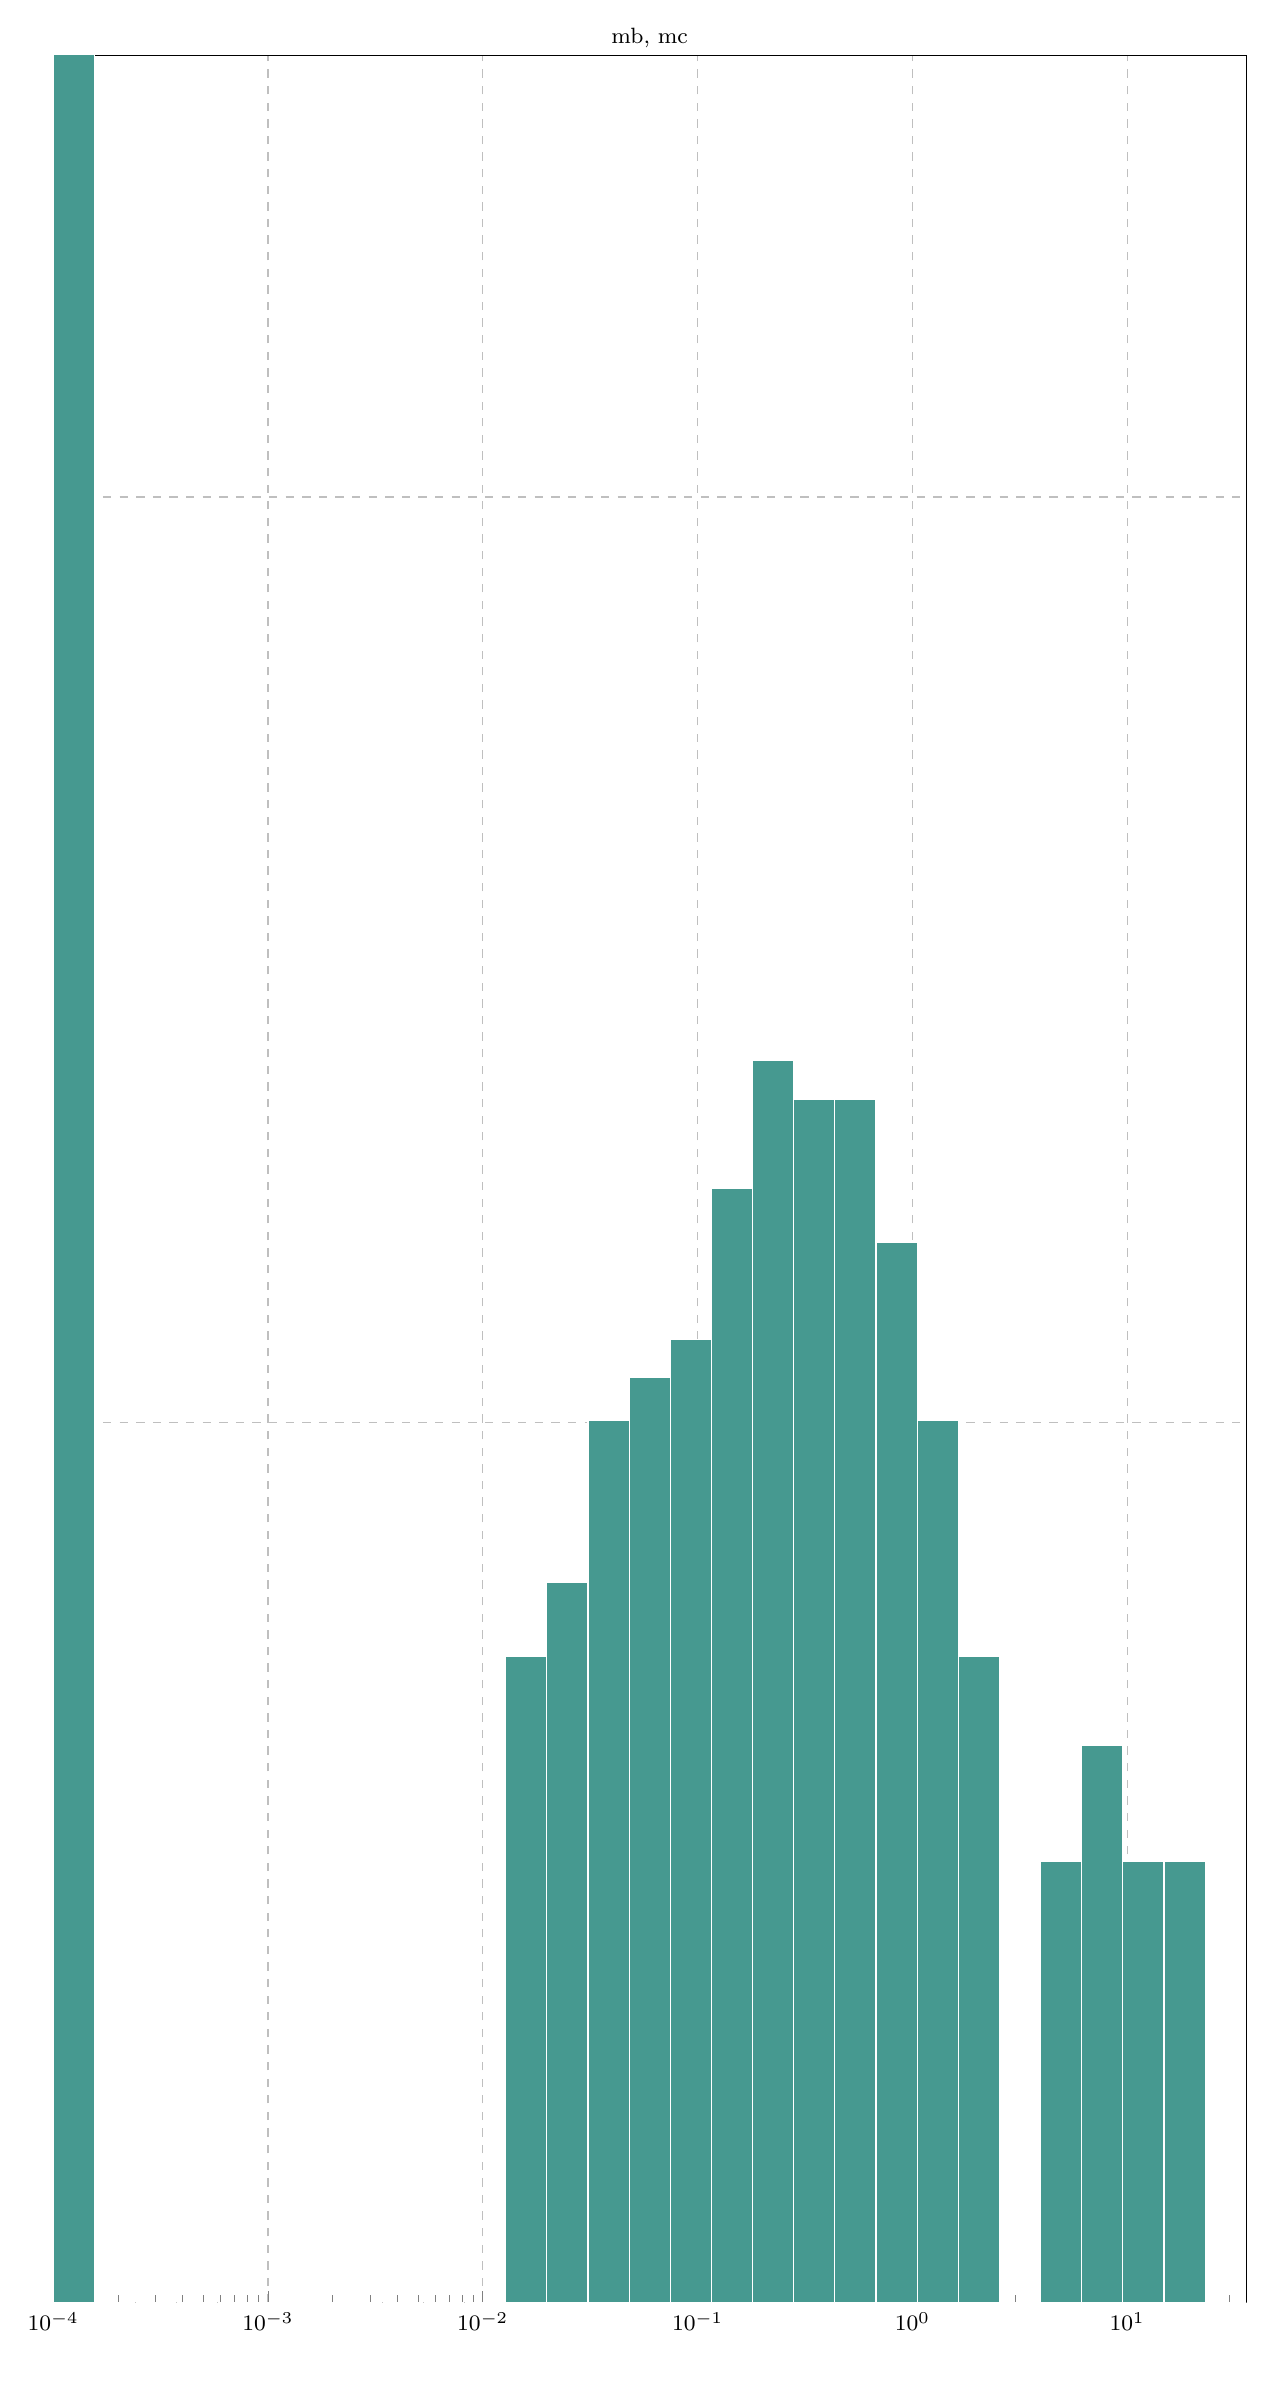
\begin{tikzpicture}

\definecolor{color0}{rgb}{0.274509803921569,0.6,0.564705882352941}

\begin{axis}[
axis line style={white!80!black},
log basis x={10},
tick pos=left,
title={frac\_batch\_exact, one\_group, N=128, D=895210},
xlabel={eigenvalues},
xmin=0.0001, xmax=35.8794860839844,
xmode=log,
ylabel={density},
ymin=1.11705508533742e-06, ymax=1,
ymode=log,
zmystyle
]
\draw[draw=white,fill=color0] (axis cs:0.0001,1.11705508533742e-06) rectangle (axis cs:0.000155434142340701,0.999840260942811);
\draw[draw=white,fill=color0] (axis cs:0.000155434142340701,1.11705508533742e-06) rectangle (axis cs:0.000241597726051892,1.11705508533742e-06);
\draw[draw=white,fill=color0] (axis cs:0.000241597726051892,1.11705508533742e-06) rectangle (axis cs:0.000375525353403394,1.11705508533742e-06);
\draw[draw=white,fill=color0] (axis cs:0.000375525353403394,1.11705508533742e-06) rectangle (axis cs:0.00058369461233445,1.11705508533742e-06);
\draw[draw=white,fill=color0] (axis cs:0.00058369461233445,1.11705508533742e-06) rectangle (axis cs:0.000907260714570931,1.11705508533742e-06);
\draw[draw=white,fill=color0] (axis cs:0.000907260714570931,1.11705508533742e-06) rectangle (axis cs:0.00141019291048744,1.11705508533742e-06);
\draw[draw=white,fill=color0] (axis cs:0.00141019291048744,1.11705508533742e-06) rectangle (axis cs:0.00219192125576551,1.11705508533742e-06);
\draw[draw=white,fill=color0] (axis cs:0.00219192125576551,1.11705508533742e-06) rectangle (axis cs:0.00340699400468264,1.11705508533742e-06);
\draw[draw=white,fill=color0] (axis cs:0.00340699400468264,1.11705508533742e-06) rectangle (axis cs:0.00529563191077756,1.11705508533742e-06);
\draw[draw=white,fill=color0] (axis cs:0.00529563191077756,1.11705508533742e-06) rectangle (axis cs:0.00823122004203757,1.11705508533742e-06);
\draw[draw=white,fill=color0] (axis cs:0.00823122004203757,1.11705508533742e-06) rectangle (axis cs:0.0127941262765169,1.11705508533742e-06);
\draw[draw=white,fill=color0] (axis cs:0.0127941262765169,1.11705508533742e-06) rectangle (axis cs:0.0198864404478903,5.58528041795857e-06);
\draw[draw=white,fill=color0] (axis cs:0.0198864404478903,1.11705508533742e-06) rectangle (axis cs:0.0309103181522725,6.70233675105834e-06);
\draw[draw=white,fill=color0] (axis cs:0.0309103181522725,1.11705508533742e-06) rectangle (axis cs:0.0480451879147667,1.00535057505797e-05);
\draw[draw=white,fill=color0] (axis cs:0.0480451879147667,1.11705508533742e-06) rectangle (axis cs:0.0746786257712956,1.11705620837905e-05);
\draw[draw=white,fill=color0] (axis cs:0.0746786257712956,1.11705508533742e-06) rectangle (axis cs:0.116076081479435,1.22876184168903e-05);
\draw[draw=white,fill=color0] (axis cs:0.116076081479435,1.11705508533742e-06) rectangle (axis cs:0.180421861710252,1.78729000826112e-05);
\draw[draw=white,fill=color0] (axis cs:0.180421861710252,1.11705508533742e-06) rectangle (axis cs:0.280437173344456,2.45752380816539e-05);
\draw[draw=white,fill=color0] (axis cs:0.280437173344456,1.11705508533742e-06) rectangle (axis cs:0.435895115192459,2.23411254152324e-05);
\draw[draw=white,fill=color0] (axis cs:0.435895115192459,1.11705508533742e-06) rectangle (axis cs:0.677529833804408,2.23411254153434e-05);
\draw[draw=white,fill=color0] (axis cs:0.677529833804408,1.11705508533742e-06) rectangle (axis cs:1.05311268627626,1.56387874163006e-05);
\draw[draw=white,fill=color0] (axis cs:1.05311268627626,1.11705508533742e-06) rectangle (axis cs:1.63689667179461,1.00535057505797e-05);
\draw[draw=white,fill=color0] (axis cs:1.63689667179461,1.11705508533742e-06) rectangle (axis cs:2.54429630280743,5.58528041795857e-06);
\draw[draw=white,fill=color0] (axis cs:2.54429630280743,1.11705508533742e-06) rectangle (axis cs:3.95470513687488,1.11705508533742e-06);
\draw[draw=white,fill=color0] (axis cs:3.95470513687488,1.11705508533742e-06) rectangle (axis cs:6.1469620116051,3.351167751648e-06);
\draw[draw=white,fill=color0] (axis cs:6.14696201160511,1.11705508533742e-06) rectangle (axis cs:9.55447768274709,4.46822408485879e-06);
\draw[draw=white,fill=color0] (axis cs:9.55447768274709,1.11705508533742e-06) rectangle (axis cs:14.8509204413116,3.351167751648e-06);
\draw[draw=white,fill=color0] (axis cs:14.8509204413116,1.11705508533742e-06) rectangle (axis cs:23.0834008176524,3.351167751648e-06);
\draw[draw=white,fill=color0] (axis cs:23.0834008176524,1.11705508533742e-06) rectangle (axis cs:35.8794860839844,1.11705508533742e-06);
\end{axis}

\end{tikzpicture}

  \end{minipage}
  \hspace{-3.5ex}
  \begin{minipage}[t]{0.33\linewidth}
    \centering
    % load "spectrumdefault{left, center, right}" styles
    % defines the pgfplots styles "spectrumdefault", "spectrumdefaultleft",
% "spectrumdefaultcenter", "spectrumdefaultright"
% pgfplots style "spectrumdefault"
\pgfkeys{/pgfplots/spectrumdefault/.style={
    width=1.38\linewidth,
    height=1.38*1.8\linewidth,
    every axis plot/.append style={line width = 1.5pt},
    tick pos = left,
    xmajorticks = true,
    ymajorticks = true,
    ylabel near ticks,
    xlabel near ticks,
    xtick align = inside,
    ytick align = inside,
    legend cell align = left,
    legend columns = 1,
    legend pos = north west,
    legend style = {
      fill opacity = 0.7,
      text opacity = 1,
      font = \footnotesize,
    },
    xticklabel style = {font = \footnotesize, inner xsep = 0ex},
    xlabel style = {font = \footnotesize},
    axis line style = {black},
    yticklabel style = {font = \footnotesize, inner ysep = 0ex},
    ylabel style = {font = \footnotesize, inner ysep = 0ex},
    title style = {font = \footnotesize, inner ysep = 0ex, yshift = -0.75ex},
    grid = major,
    grid style = {dashed}
  }
}
% pgfplots style for left "spectrumdefaultleft"
\pgfkeys{/pgfplots/spectrumdefaultleft/.style={
    spectrumdefault,
    title=\empty,
    ymax=3e-4,
    xlabel=\phantom{eigenvalues},
  }}
% pgfplots style for center "spectrumdefaultcenter"
\pgfkeys{/pgfplots/spectrumdefaultcenter/.style={
    spectrumdefault,
    ylabel=\empty,
    yticklabels=\empty,
    title=\empty,
    ymax=3e-4,
  }}
% pgfplots style for right "spectrumdefaultright"
\pgfkeys{/pgfplots/spectrumdefaultright/.style={
    spectrumdefault,
    ylabel=\empty,
    yticklabels=\empty,
    title=\empty,
    ymax=3e-4,
    xlabel=\phantom{eigenvalues},
  }}

%%% Local Variables:
%%% mode: latex
%%% TeX-master: "../../thesis"
%%% End:

    % customize "zmystyle" as you wish
    \pgfkeys{/pgfplots/zmystyle/.style={spectrumdefaultright,
        title={mb, mc}}}
    % This file was created by tikzplotlib v0.9.7.
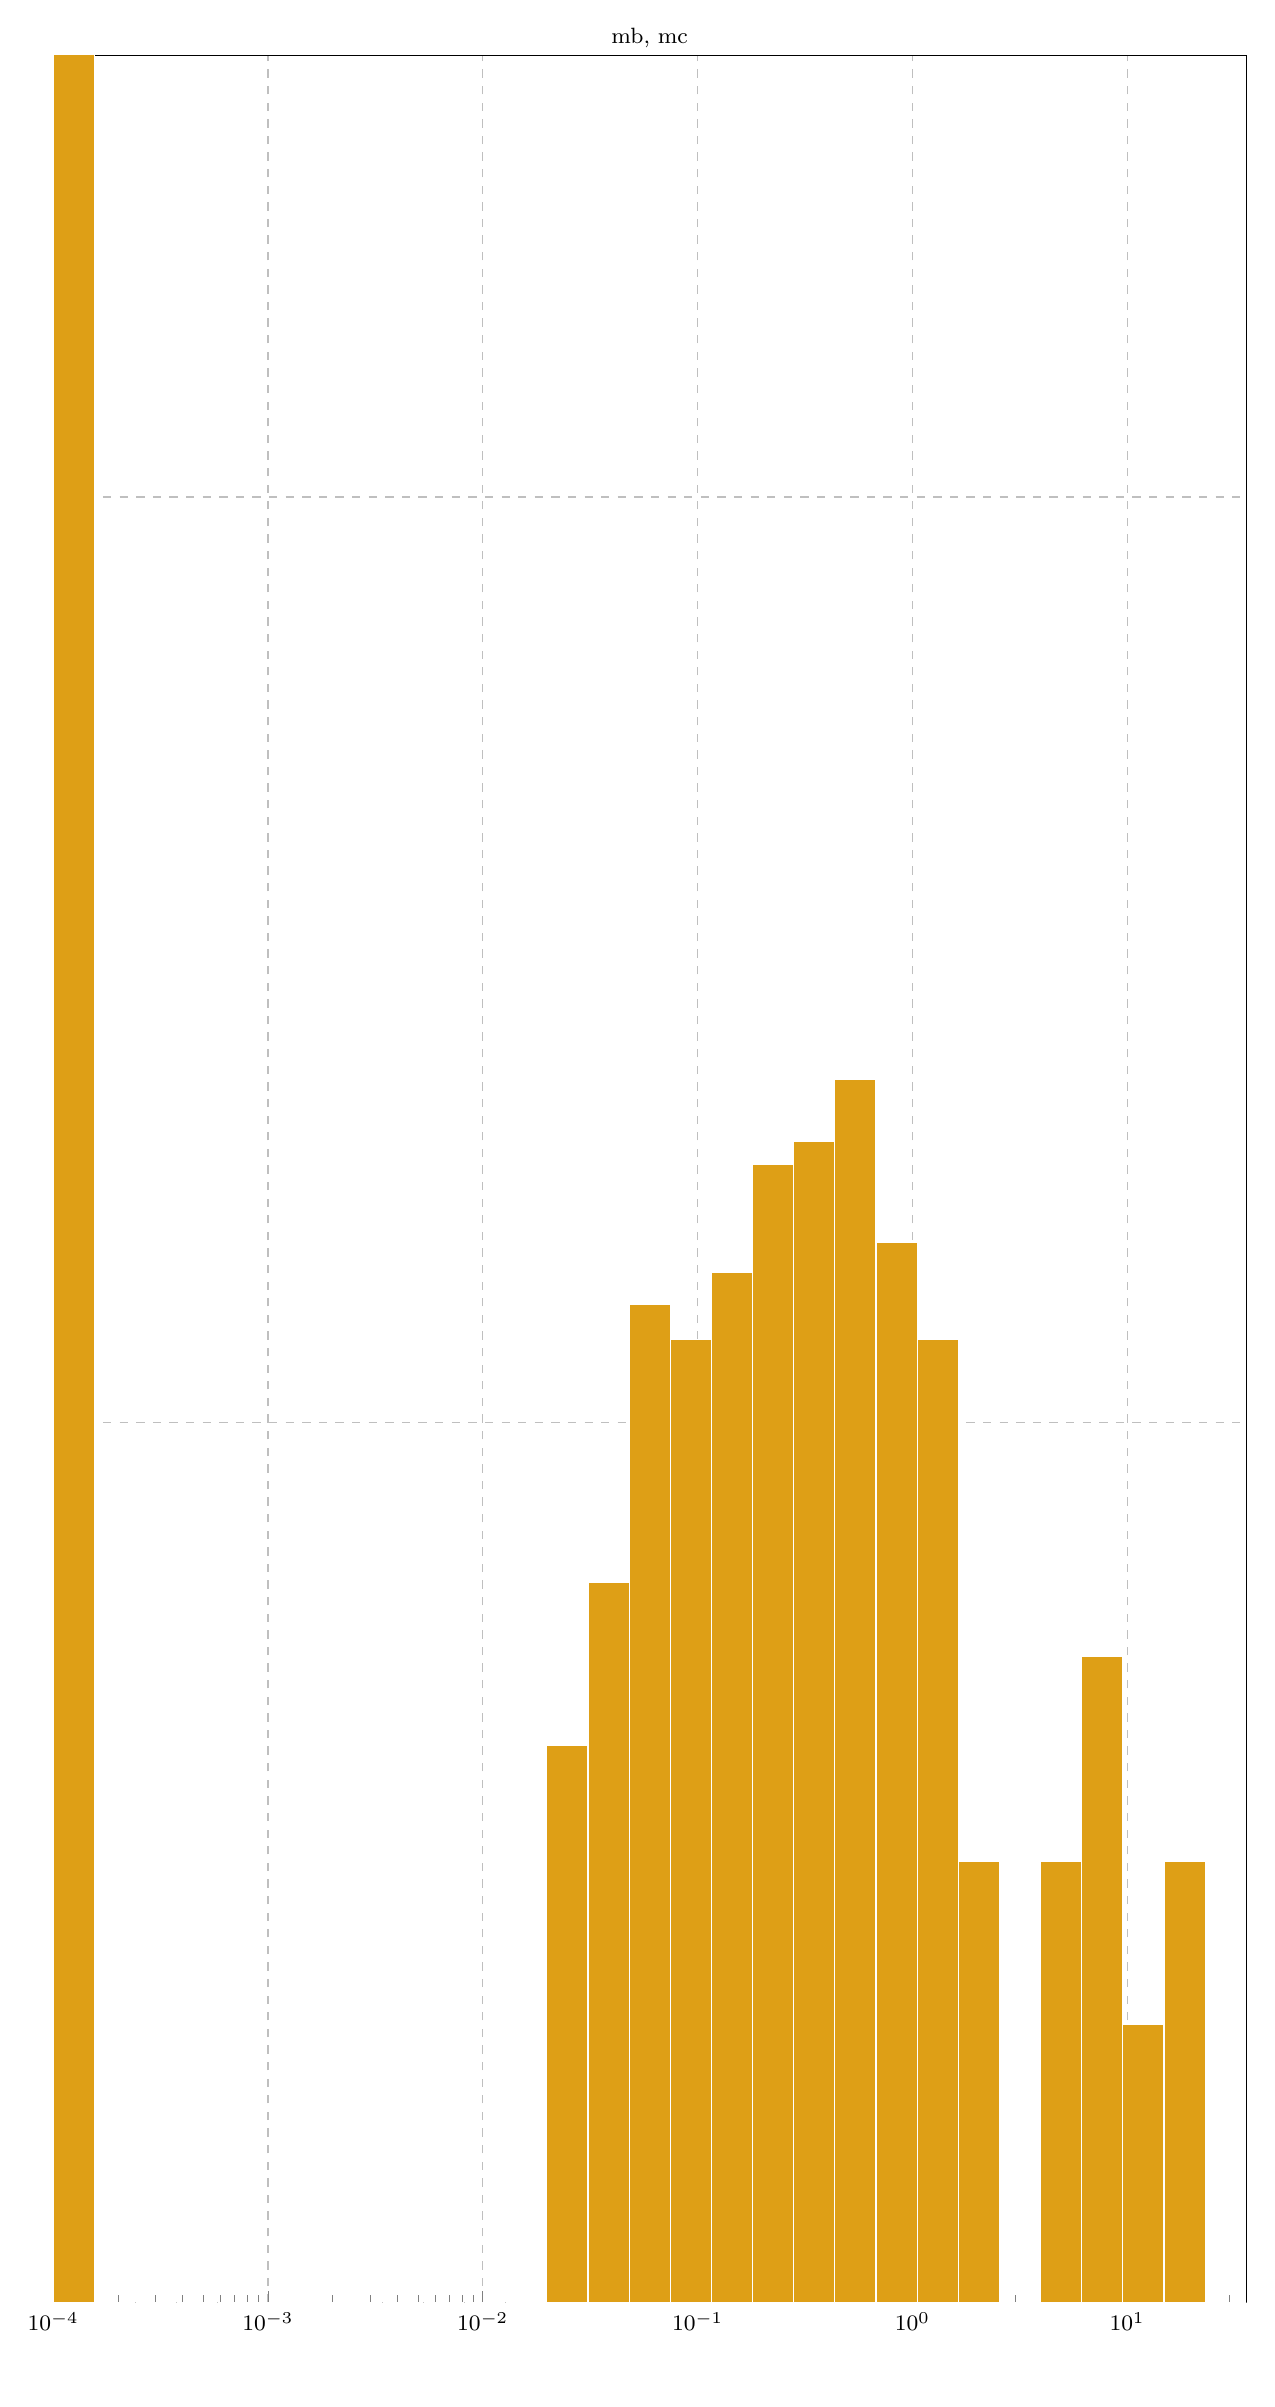
\begin{tikzpicture}

\definecolor{color0}{rgb}{0.870588235294118,0.623529411764706,0.0862745098039216}

\begin{axis}[
axis line style={white!80!black},
log basis x={10},
tick pos=left,
title={full\_batch\_mc, one\_group, N=128, D=895210},
xlabel={eigenvalues},
xmin=0.0001, xmax=35.8794860839844,
xmode=log,
ylabel={density},
ymin=1.11705508533742e-06, ymax=1,
ymode=log,
zmystyle
]
\draw[draw=white,fill=color0] (axis cs:0.0001,1.11705508533742e-06) rectangle (axis cs:0.000155434142340701,0.999858133844141);
\draw[draw=white,fill=color0] (axis cs:0.000155434142340701,1.11705508533742e-06) rectangle (axis cs:0.000241597726051892,1.11705508533742e-06);
\draw[draw=white,fill=color0] (axis cs:0.000241597726051892,1.11705508533742e-06) rectangle (axis cs:0.000375525353403394,1.11705508533742e-06);
\draw[draw=white,fill=color0] (axis cs:0.000375525353403394,1.11705508533742e-06) rectangle (axis cs:0.00058369461233445,1.11705508533742e-06);
\draw[draw=white,fill=color0] (axis cs:0.00058369461233445,1.11705508533742e-06) rectangle (axis cs:0.000907260714570931,1.11705508533742e-06);
\draw[draw=white,fill=color0] (axis cs:0.000907260714570931,1.11705508533742e-06) rectangle (axis cs:0.00141019291048744,1.11705508533742e-06);
\draw[draw=white,fill=color0] (axis cs:0.00141019291048744,1.11705508533742e-06) rectangle (axis cs:0.00219192125576551,1.11705508533742e-06);
\draw[draw=white,fill=color0] (axis cs:0.00219192125576551,1.11705508533742e-06) rectangle (axis cs:0.00340699400468264,1.11705508533742e-06);
\draw[draw=white,fill=color0] (axis cs:0.00340699400468264,1.11705508533742e-06) rectangle (axis cs:0.00529563191077756,1.11705508533742e-06);
\draw[draw=white,fill=color0] (axis cs:0.00529563191077756,1.11705508533742e-06) rectangle (axis cs:0.00823122004203757,1.11705508533742e-06);
\draw[draw=white,fill=color0] (axis cs:0.00823122004203757,1.11705508533742e-06) rectangle (axis cs:0.0127941262765169,1.11705508533742e-06);
\draw[draw=white,fill=color0] (axis cs:0.0127941262765169,1.11705508533742e-06) rectangle (axis cs:0.0198864404478903,1.11705508533742e-06);
\draw[draw=white,fill=color0] (axis cs:0.0198864404478903,1.11705508533742e-06) rectangle (axis cs:0.0309103181522725,4.46822408474777e-06);
\draw[draw=white,fill=color0] (axis cs:0.0309103181522725,1.11705508533742e-06) rectangle (axis cs:0.0480451879147667,6.70233675116937e-06);
\draw[draw=white,fill=color0] (axis cs:0.0480451879147667,1.11705508533742e-06) rectangle (axis cs:0.0746786257712956,1.34046747499901e-05);
\draw[draw=white,fill=color0] (axis cs:0.0746786257712956,1.11705508533742e-06) rectangle (axis cs:0.116076081479435,1.22876184168903e-05);
\draw[draw=white,fill=color0] (axis cs:0.116076081479435,1.11705508533742e-06) rectangle (axis cs:0.180421861710252,1.45217310832009e-05);
\draw[draw=white,fill=color0] (axis cs:0.180421861710252,1.11705508533742e-06) rectangle (axis cs:0.280437173344456,1.8989956415822e-05);
\draw[draw=white,fill=color0] (axis cs:0.280437173344456,1.11705508533742e-06) rectangle (axis cs:0.435895115192459,2.01070127490328e-05);
\draw[draw=white,fill=color0] (axis cs:0.435895115192459,1.11705508533742e-06) rectangle (axis cs:0.677529833804408,2.34581817484432e-05);
\draw[draw=white,fill=color0] (axis cs:0.677529833804408,1.11705508533742e-06) rectangle (axis cs:1.05311268627626,1.56387874163006e-05);
\draw[draw=white,fill=color0] (axis cs:1.05311268627626,1.11705508533742e-06) rectangle (axis cs:1.63689667179461,1.22876184168903e-05);
\draw[draw=white,fill=color0] (axis cs:1.63689667179461,1.11705508533742e-06) rectangle (axis cs:2.54429630280743,3.351167751648e-06);
\draw[draw=white,fill=color0] (axis cs:2.54429630280743,1.11705508533742e-06) rectangle (axis cs:3.95470513687488,1.11705508533742e-06);
\draw[draw=white,fill=color0] (axis cs:3.95470513687488,1.11705508533742e-06) rectangle (axis cs:6.1469620116051,3.351167751648e-06);
\draw[draw=white,fill=color0] (axis cs:6.14696201160511,1.11705508533742e-06) rectangle (axis cs:9.55447768274709,5.58528041795857e-06);
\draw[draw=white,fill=color0] (axis cs:9.55447768274709,1.11705508533742e-06) rectangle (axis cs:14.8509204413116,2.23411141854822e-06);
\draw[draw=white,fill=color0] (axis cs:14.8509204413116,1.11705508533742e-06) rectangle (axis cs:23.0834008176524,3.351167751648e-06);
\draw[draw=white,fill=color0] (axis cs:23.0834008176524,1.11705508533742e-06) rectangle (axis cs:35.8794860839844,1.11705508533742e-06);
\end{axis}

\end{tikzpicture}

  \end{minipage}
  \end{subfigure}
  \hfill
  \begin{subfigure}{0.44\linewidth}
    \centering
    \vspace{-4.7ex}
    \caption{}
    \label{subfig:visual_abstract_2}
    \vspace{-0.8\baselineskip}
    \begin{tikzpicture}
  % PDF Picture. Set the origin to the south west corner
  \node[inner sep=0pt] (pdf_plot) at (0,0){\includegraphics[width=\linewidth]{fig/visual_abstract/vivit_quantities_transparent.pdf}};

  \coordinate (origin) at (pdf_plot.south west);

  % Text
  \node[anchor=south west, inner sep=0pt] at ($ (origin) + (0.25*\linewidth, 0.26*\linewidth)$)
  {$\vtheta_t$};

  \node[anchor=south west, inner sep=0pt] at ($ (origin) + (0.5*\linewidth, 0.26*\linewidth) $)
  {$\textcolor{oo_gelb}{\ve_k}$};

  \node[anchor=south west, inner sep=0pt] at ($ (origin) + (0.85*\linewidth, 0.6*\linewidth) $)
  {$\textcolor{oo_rot}{\gL}$};

  \node[anchor=south west, inner sep=0pt] at ($ (origin) + (0.85*\linewidth, 0.37*\linewidth) $)
  {$\textcolor{oo_blau}{q}$};

  \node[anchor=south west, inner sep=0pt] at ($ (origin) + (0.26*\linewidth, 0.6*\linewidth) $)
  {$\textcolor{oo_gelb}{\mathcal{E}}$};

  \node[anchor=south west, inner sep=0pt, rotate=21] at ($ (origin) + (0.66*\linewidth, 0.035*\linewidth) $)
  {$\textcolor{oo_blau}{\gamma_k} ,\textcolor{oo_blau}{\lambda_k}$};

  \node[anchor=south west, inner sep=0pt, rotate=30] at ($ (origin) + (0.8*\linewidth, -0.02*\linewidth) $)
  {$\textcolor{oo_gruen}{\gamma_{nk}} ,\textcolor{oo_gruen}{\lambda_{nk}}$};
\end{tikzpicture}

%%% Local Variables:
%%% mode: latex
%%% TeX-master: "../main"
%%% End:

    \vspace{-0.5\baselineskip}
  \end{subfigure}

  \vspace{-3.0ex}

  \caption{
  \textbf{Overview of \vivittitle's quantities:}
\textbf{(a)} \ggn eigenvalue distribution of \deepobs' \threecthreed architecture on
\cifarten \cite{schneider2019deepobs}
% ($D = 895,210$, $C = 10$)
for settings with different costs on a mini-batch of size $N = 128$.
From left to right: Exact \ggn,
% on the mini-batch,
exact GGN on a mini-batch fraction,
% ($\nicefrac{1}{8}$, as in \cite{zhang2017blockdiagonal}),
\mc approximation of the \ggn.
% on the mini-batch.
%
\textbf{(b)} Pictorial illustration: Loss function $\textcolor{oo_rot}{\gL}$
from \Cref{eq:objective-function} and quadratic model $\textcolor{oo_blau}{q}$
around $\vtheta_t \in \mathbb{R}^2$ from \Cref{eq:quadratic_model} (both
represented by their contour lines). The low-rank structure provides efficient
access to the \ggn{}'s eigenvectors $\{\textcolor{oo_gelb}{\ve_k}\}$, along
which $\textcolor{oo_blau}{q}$ decouples into one-dimensional parabolas
characterized by the directional derivatives $\textcolor{oo_blau}{\gamma_k},
\textcolor{oo_blau}{\lambda_k}$ and per-sample contributions
$\textcolor{oo_gruen}{\gamma_{nk}}, \textcolor{oo_gruen}{\lambda_{nk}}$
(\Cref{eq:gammas-lambdas}). $\textcolor{oo_gelb}{\mathcal{E}}$ is the \ggn{}'s
top-$1$ eigenspace.}
  \label{fig:visual_abstract}
\end{figure}

%%% Local Variables:
%%% mode: latex
%%% TeX-master: "../main"
%%% End:
